\chapter{Risultati sperimentali} % (fold)
\label{chap:Risultati sperimentali}

\section{Addestramento} % (fold)
\label{sec:Addestramento}

Il modello \`e stato addestrato mediante l'uso della \textit{cross-validation}(\autoref{fig:cross_validation})
con una suddivisione dei dati in 5 parti uguali(5 folds).

Essendo una tipologia di apprendimento supervisionata, al modello sono fornite immagini
originali e le loro segmentazioni effettuate manualemte.

\begin{figure}[!ht]
	\begin{adjustbox}{width=0.7\columnwidth, center}
    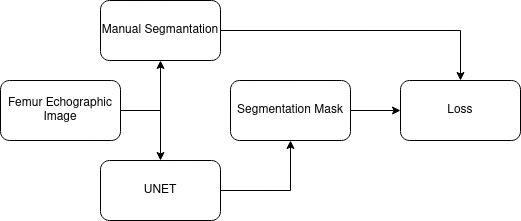
\includegraphics{./images/training.png}
  \end{adjustbox}
  \caption{Addestramento del modello}
  \label{fig:addestramento del modello}
\end{figure}

Effettuando l'addestramento con 5 folds, il modello viene addestrato 5 volte, ogni volta con un fold diverso,
l'errore finale \`e dato dalla media degli errori ottenuti dalle 5 iterazioni.

\begin{figure}[!ht]
	\begin{adjustbox}{width=0.9\columnwidth, center}
    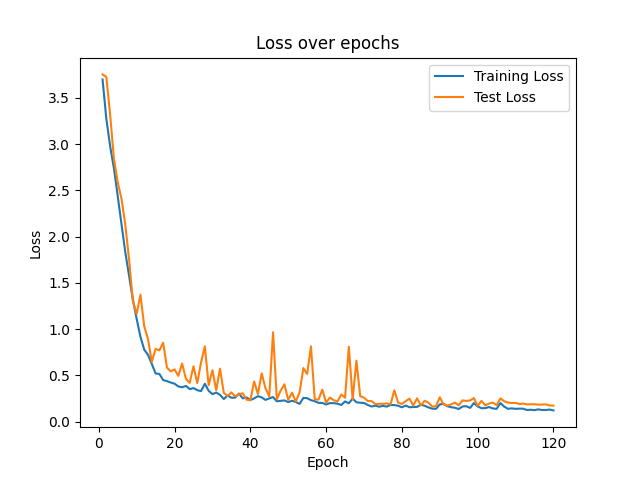
\includegraphics{./images/fold_0_loss.png} 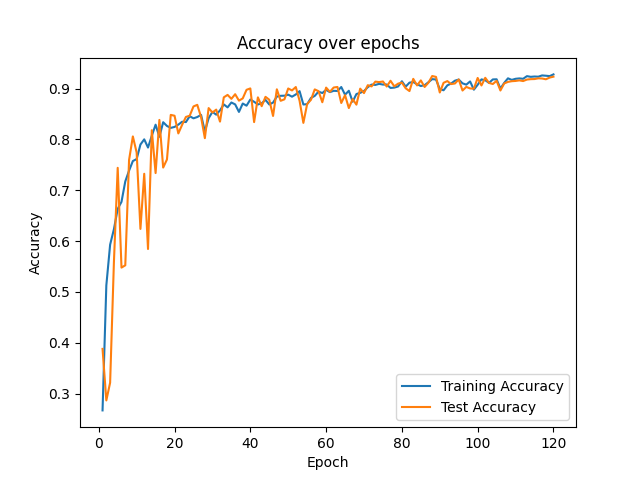
\includegraphics{./images/fold_0_accuracy.png}
  \end{adjustbox}
  \caption{Errore e accuratezza della prima porzione di dati}
  \label{fig:loss e accuratezza della prima porzione di dati}
\end{figure}

\begin{figure}[!ht]
	\begin{adjustbox}{width=0.9\columnwidth, center}
    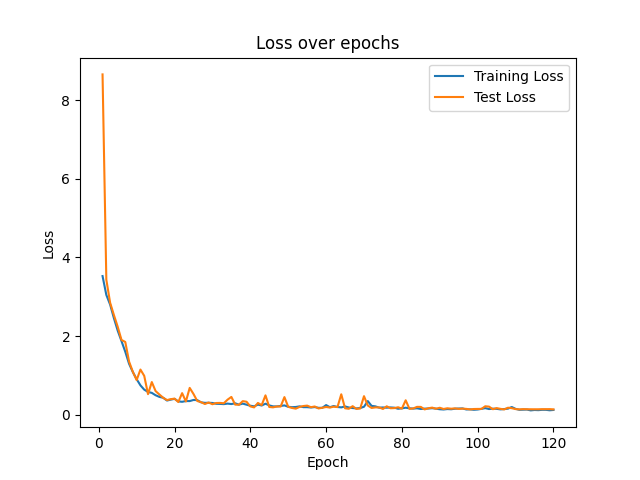
\includegraphics{./images/fold_1_loss.png} 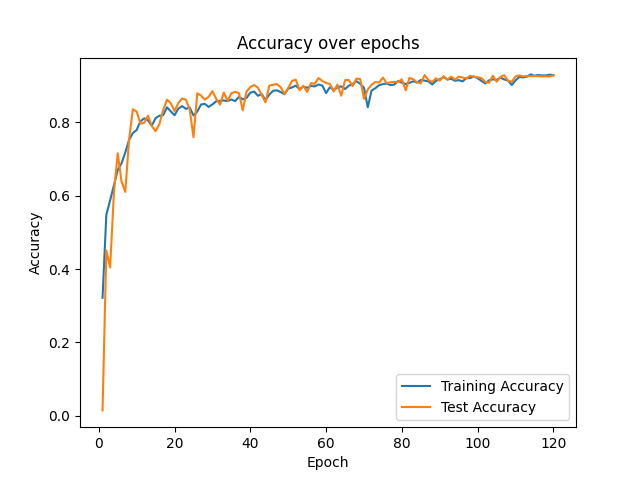
\includegraphics{./images/fold_1_accuracy.png}
  \end{adjustbox}
  \caption{Errore e accuratezza della seconda porzione di dati}
  \label{fig:loss e accuratezza della seconda porzione di dati}
\end{figure}

\begin{figure}[!ht]
	\begin{adjustbox}{width=0.9\columnwidth, center}
    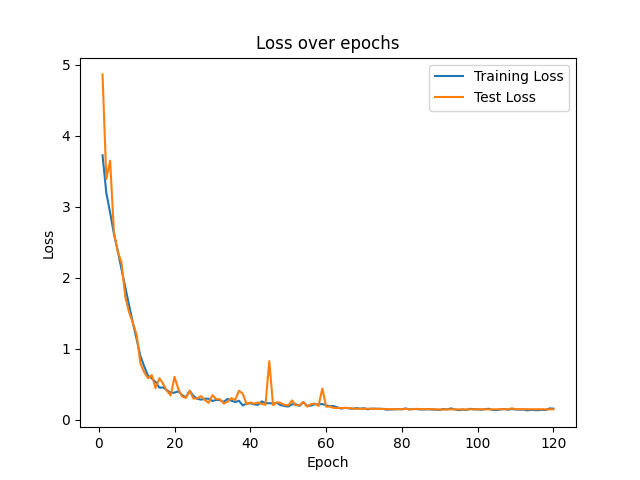
\includegraphics{./images/fold_2_loss.png} 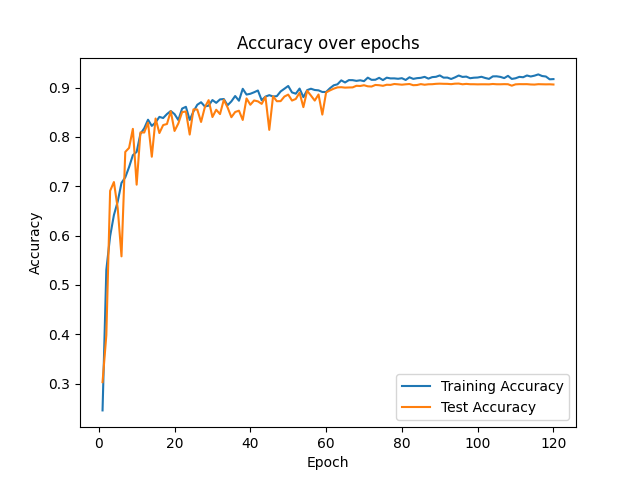
\includegraphics{./images/fold_2_accuracy.png}
  \end{adjustbox}
  \caption{Errore e accuratezza della terza porzione di dati}
  \label{fig:loss e accuratezza della terza porzione di dati}
\end{figure}

\begin{figure}[!ht]
	\begin{adjustbox}{width=0.9\columnwidth, center}
    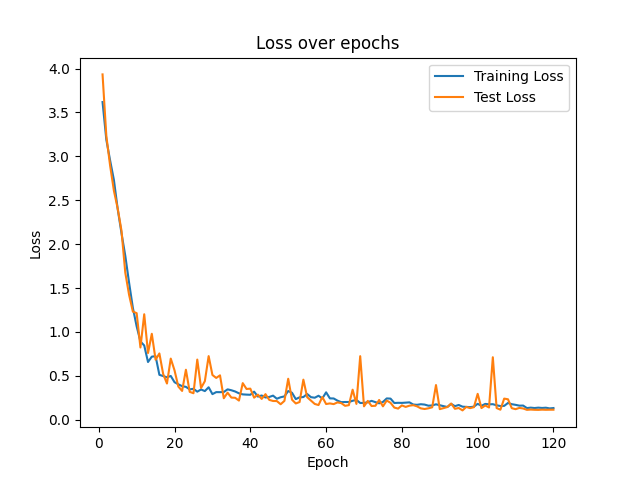
\includegraphics{./images/fold_3_loss.png} 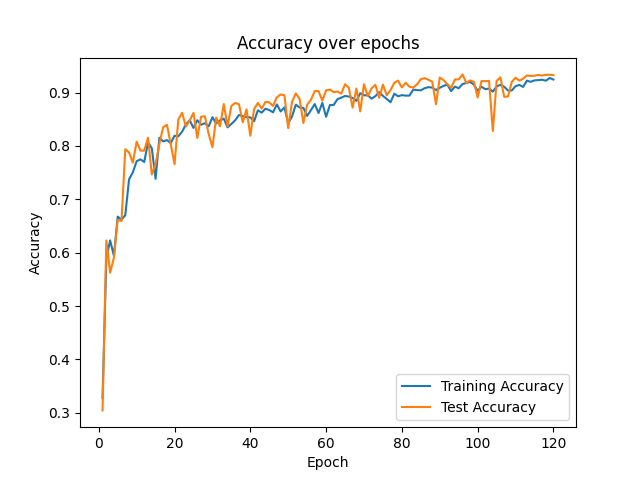
\includegraphics{./images/fold_3_accuracy.png}
  \end{adjustbox}
  \caption{Errore e accuratezza della quarta porzione di dati}
  \label{fig:loss e accuratezza della quarta porzione di dati}
\end{figure}

\begin{figure}[!ht]
	\begin{adjustbox}{width=0.9\columnwidth, center}
    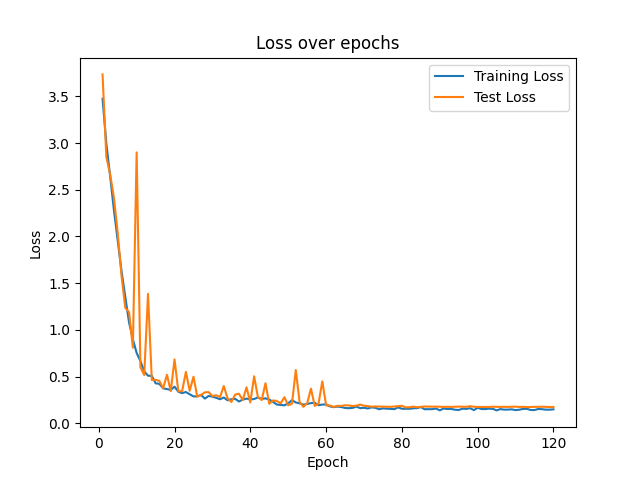
\includegraphics{./images/fold_4_loss.png} 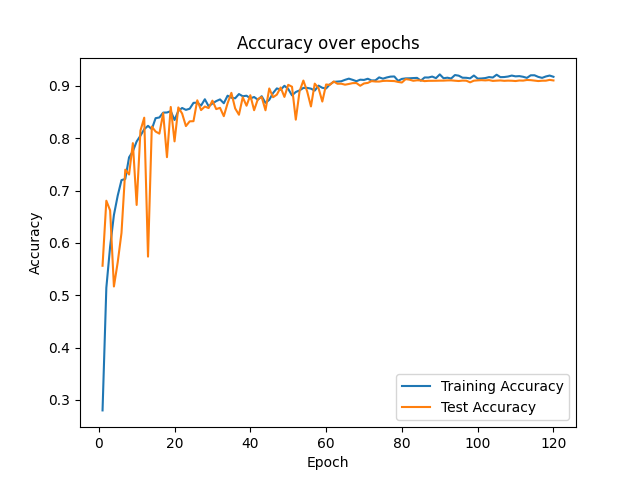
\includegraphics{./images/fold_4_accuracy.png}
  \end{adjustbox}
  \caption{Errore e accuratezza della quinta porzione di dati}
  \label{fig:loss e accuratezza della quinta porzione di dati}
\end{figure}

L'\textbf{errore} medio del modello \`e di \textbf{$8\%$} mentre l'\textbf{accuratezza} media \`e di \textbf{$92\%$}(le metriche utilizzate \autoref{sec:metriche}).



Considerando che questo modello \`e stato utilizzato in ambito medico per velocizzare e standardizzare 
la segmentazione dei femori per un'analisi su questi ultimi, oltre ad analisi quantitative, \`e stato 
necessario effettuare delle analisi qualitative sulal segmentazione ottenuta dal modello.

Nelle immagini seguenti viene riportato uno delle immagini prese in considerazione per l'addestramento del modello
e vengono mostrate le segmentazione manuali, le segmentazioni ottenute dal modello e la differenze 
nella classificazione dei pixel tra le due segmentazioni.


Partendo da una immagini (\autoref{fig:immagine originale}) ottenuta mediante la raccolta dati effettuata dai medici, 

\begin{figure}[!ht]
	\begin{adjustbox}{width=0.8\columnwidth, center}
    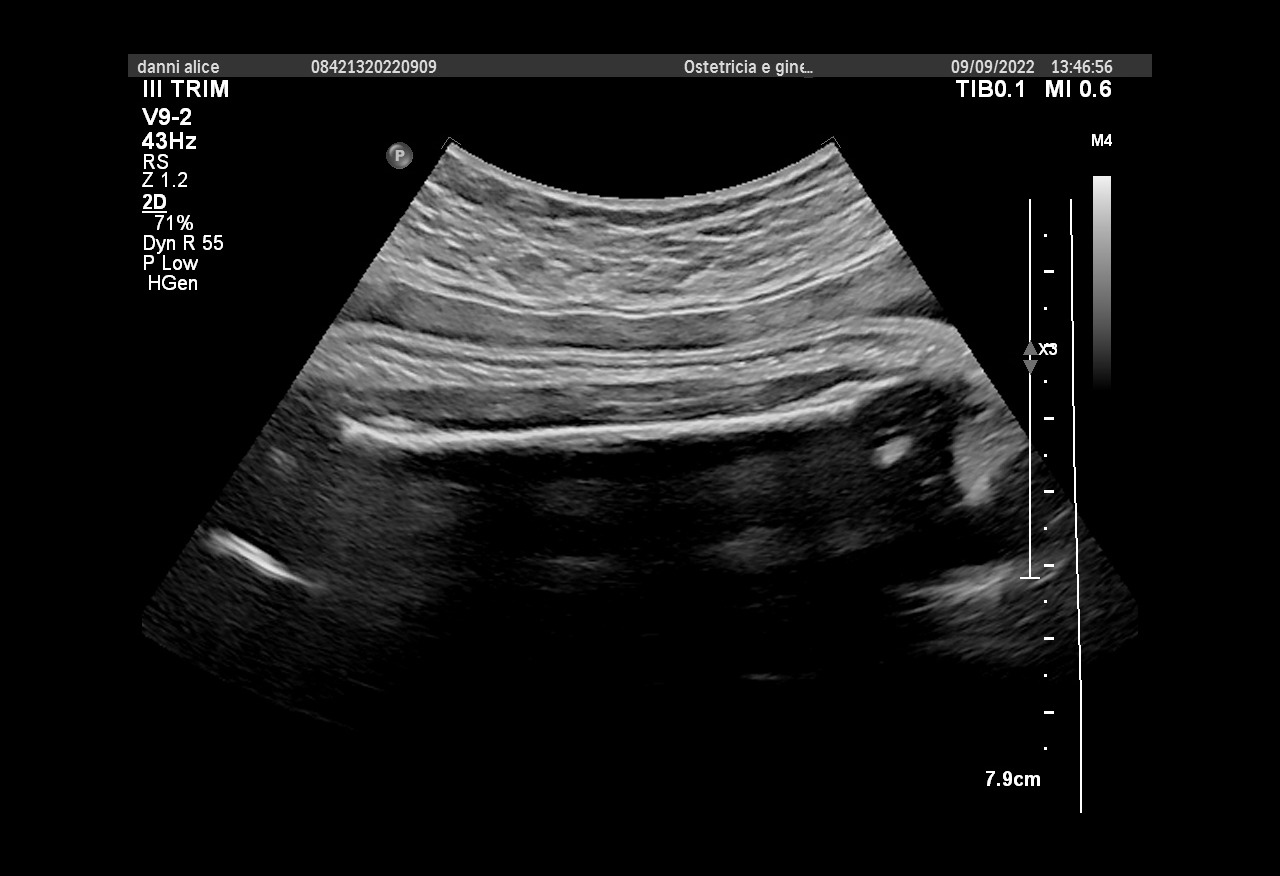
\includegraphics{./images/image.png}
  \end{adjustbox}
  \caption{Immagine originale}
  \label{fig:immagine originale}
\end{figure}

I risultati ottenuti mediante la segmentazione manuale e la segmentazione del modello sono i seguenti:
\begin{figure}[!ht]
	\begin{adjustbox}{width=0.9\columnwidth, center}
    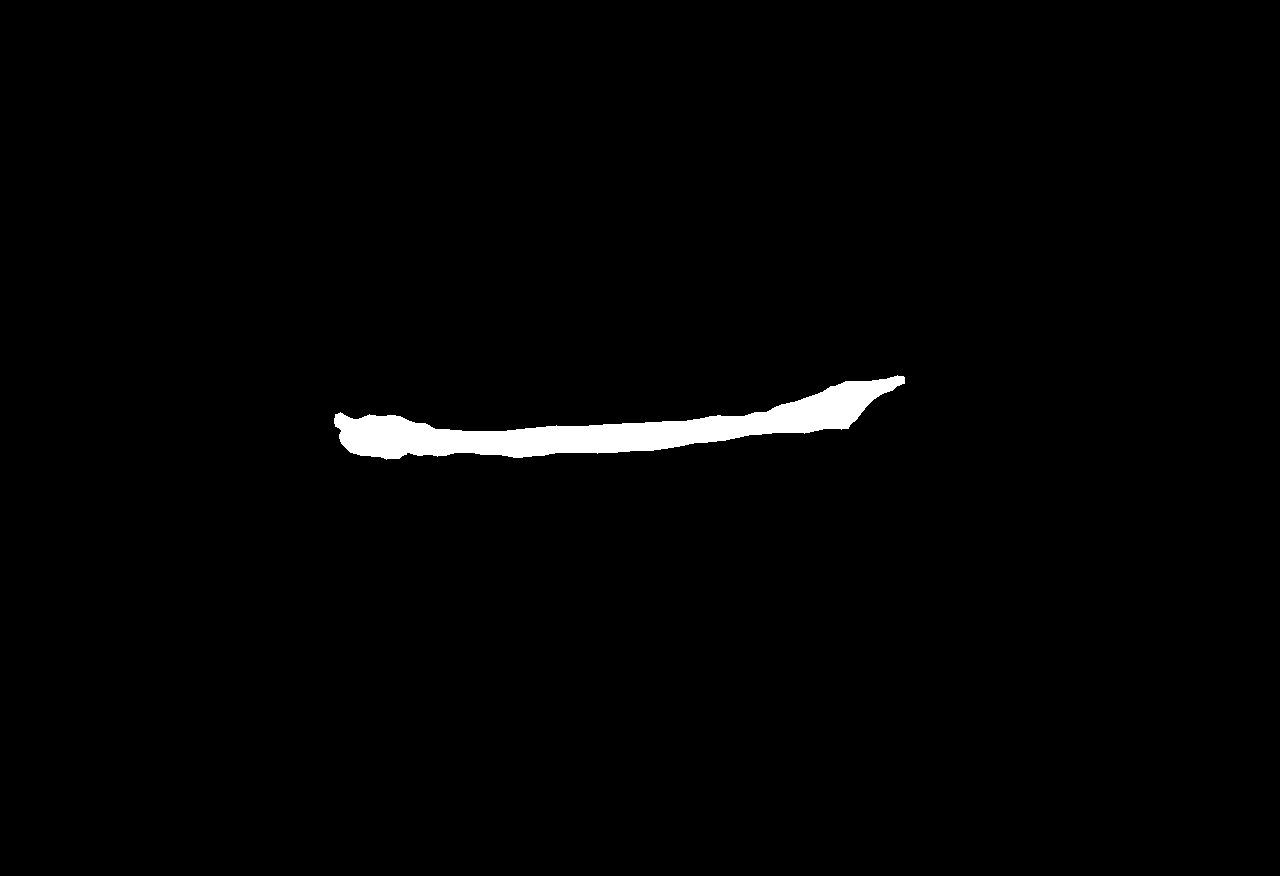
\includegraphics{./images/mask.png}
    \hspace{20pt} % Add horizontal space between the two images
    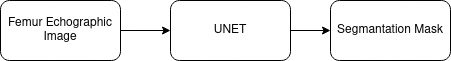
\includegraphics{./images/prediction.png}
  \end{adjustbox}
  \caption{Segmentazione manuale(sinistra) e segmentazione del modello(destra)}
  \label{fig:segmentazione manuale e segmentazione del modello}
\end{figure}


Per sostenere la tesi che il modello riesca a segmentare correttamente le immagini, \`e stata 
calcolata la distribuzione dei pixel per controntare la segmentazione manuale con quella del modello.

\begin{figure}[!ht]
	\begin{adjustbox}{width=0.9\columnwidth, center}
    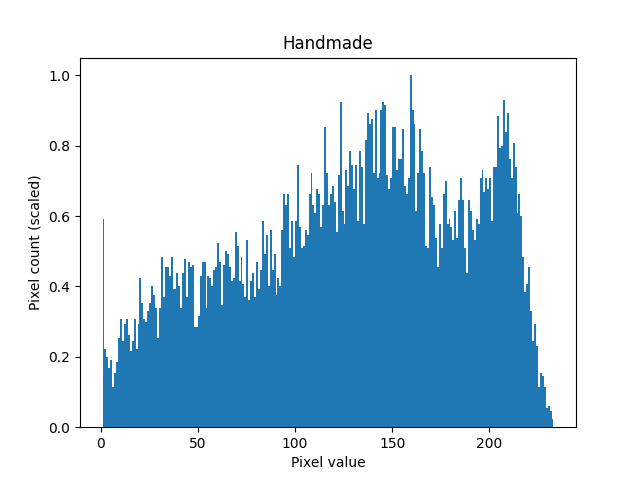
\includegraphics{./images/handmade_scaled_hist.png}
    \hspace{20pt} % Add horizontal space between the two images
    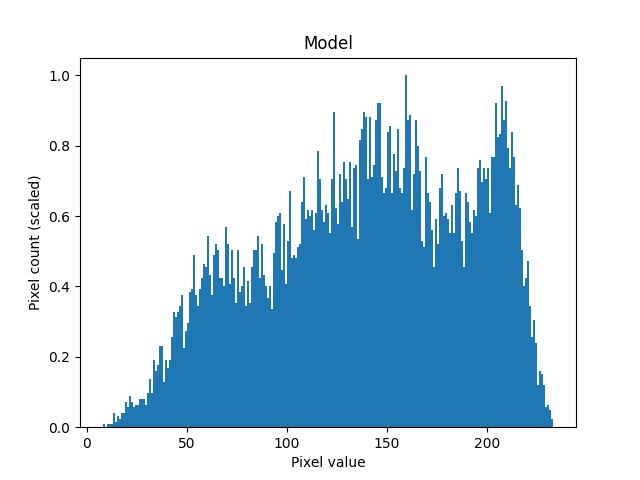
\includegraphics{./images/model_scaled_hist.png}
  \end{adjustbox}
  \caption{Distribuzione dei pixel della segmentazione manuale(sinistra) e del modello(destra)}
  \label{fig:distribuzione dei pixel della segmentazione manuale e del modello}
\end{figure}

Un'altra rappresentazione a confronto dei risultati ottenuti \`e la seguente:

\begin{figure}[!ht]
	\begin{adjustbox}{width=0.65\columnwidth, center}
    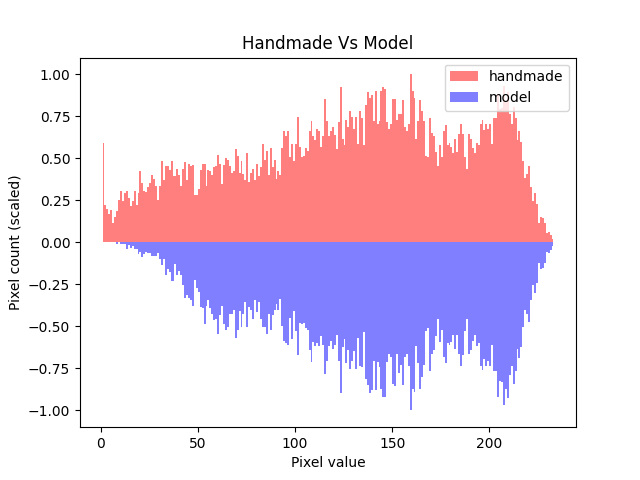
\includegraphics{./images/handmade_vs_model_scaled.png}
  \end{adjustbox}
  \caption{Confronto tra la segmentazione manuale e quella del modello}
  \label{fig:confronto tra la segmentazione manuale e quella del modello}
\end{figure}

Dai risultati qualitatitivi e quantitativi si pu\`o constatare che il modello ha una performance
molto promettente in quanto supera abbondantemente un'accuratezza del $90\%$ e pu\`o essere 
addestrato incrementando il numero di imamgini a disposizione. 

Non sono necessari ulteriori segmentazioni manuali ma si possono direttamente sfruttare
le nuove immagini raccolte, segmentarle mediante l'uso del modello e utilizzarle per l'addestramento.




% section Addestramento (end)

\section{Problema} % (fold)
\label{sec:Problema}

Il modello è stato progettato e realizzato per svolgere la segmentazione di immagini di femori fetali \cite{abstract1} \cite{abstract2} .
L'utilizzo del modello permette l'automatizzazione di un compito che altrimenti richiederebbe lo sforzo e il tempo di un 
professionista che così può svolgere altre attività meno monotone.

Nello specifico il modello è stato utilizzato per automatizzare l'estrazione dei pixel relativi al femore di un feto 
nelle settimane 35-37 di gestazione. 

I pixel estratti venivano processati per strarne la luminosità che nelle analisi ecografiche corrisponde 
alla \textbf{densità minerale ossea} o \textbf{bone mineral density}(BMD) del femore fetale
per correlarlo ai dati relativi al peso di nascita.

È stato rilevato un trend di correlazione debole tra luminosit\`a e peso alla nascita. (\autoref{fig:correlazione tra luminosità e peso alla nascita})


\begin{figure}[!ht]
	\begin{adjustbox}{width=0.7\columnwidth, center}
    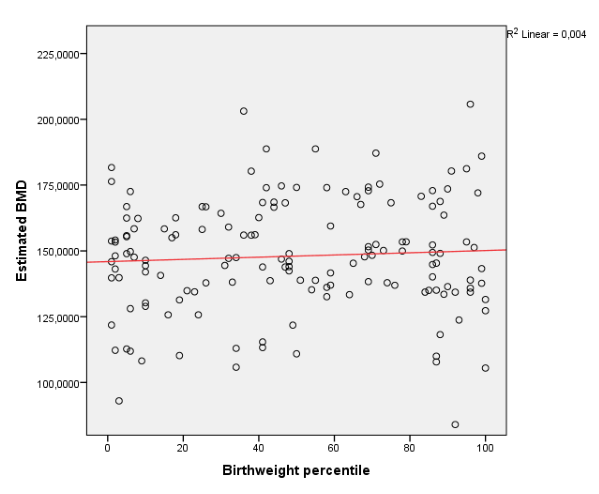
\includegraphics{./images/correlation_weight_abstract.png}
  \end{adjustbox}
  \caption{Correlazione tra luminosità e peso alla nascita}
  \label{fig:correlazione tra luminosità e peso alla nascita}
\end{figure}

La rete neurale si è dimostrata capace di riconoscere i pixels contenenti dati relativi all'area del femore, inoltre i dati prodotti dalla rete hanno portato a tenere in considerazione 
l'utilizzo della rete per analisi successive.



% chapter Risultati sperimentali (end)
